\documentclass{article}
\usepackage{amssymb}
\usepackage{tikz}

\title{Modes of Convergence}
\author{William G Underwood}

\begin{document}

\maketitle

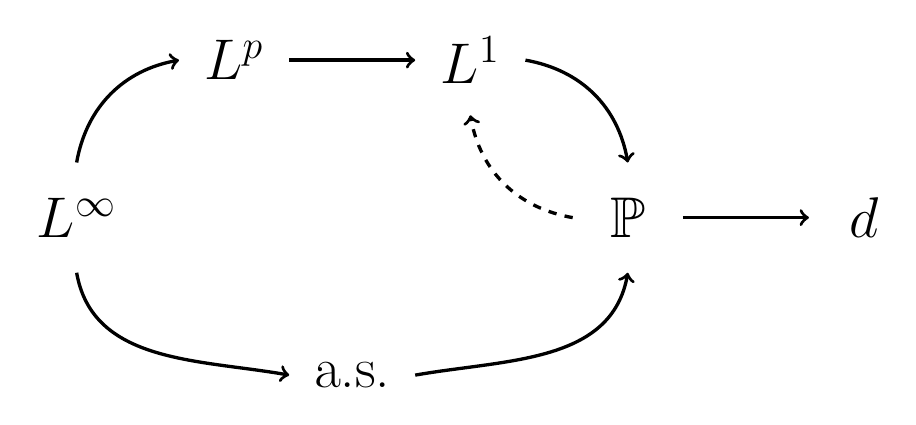
\begin{tikzpicture}

  % nodes
  \node at (0,0) {\huge $L^\infty$};
  \node at (2,2) {\huge $L^p$};
  \node at (5,2) {\huge $L^1$};
  \node at (7,0) {\huge $\mathbb{P}$};
  \node at (10,0) {\huge $d$};
  \node at (3.5,-2) {\huge a.s.};

  % arrows
  \draw [->, very thick] (0,0.7) to [out=80,in=190] (1.3,2);
  \draw [->, very thick] (2.7,2) -- (4.3,2);
  \draw [->, very thick] (5.7,2) to [out=-10,in=100] (7,0.7);
  \draw [->, very thick, dashed] (6.3,0) to [out=170,in=-80] (5,1.3);
  \draw [->, very thick] (7.7,0) -- (9.3,0);
  \draw [->, very thick] (0,-0.7) to [out=-80,in=170] (2.7,-2);
  \draw [->, very thick] (4.3,-2) to [out=10,in=-100] (7,-0.7);

\end{tikzpicture}

\end{document}